
\subsection{brnn method}\label{brnn-method}

6-layer neural network that utilizes Bayesian Regularization

predictions for a magnitude 9.1 earthquake

\hypertarget{building-the-network}{%
\subsubsection{Building the Network}\label{building-the-network}}

\begin{Shaded}
\begin{Highlighting}[]
\NormalTok{x }\OtherTok{\textless{}{-}}\NormalTok{ earthquakes\_log}\SpecialCharTok{$}\NormalTok{mag}
\NormalTok{y }\OtherTok{\textless{}{-}}\NormalTok{ earthquakes\_log}\SpecialCharTok{$}\NormalTok{freqc}

\NormalTok{brnn }\OtherTok{\textless{}{-}} \FunctionTok{brnn}\NormalTok{(y}\SpecialCharTok{\textasciitilde{}}\NormalTok{x,}\AttributeTok{neurons=}\DecValTok{6}\NormalTok{)                       }\CommentTok{\# build model}
\end{Highlighting}
\end{Shaded}

\begin{verbatim}
## Number of parameters (weights and biases) to estimate: 18 
## Nguyen-Widrow method
## Scaling factor= 4.2 
## gamma= 6.6171     alpha= 0.1129   beta= 869.274
\end{verbatim}

\begin{Shaded}
\begin{Highlighting}[]
\NormalTok{b }\OtherTok{\textless{}{-}} \FunctionTok{predict}\NormalTok{(brnn, }\AttributeTok{newdata =} \FunctionTok{data.frame}\NormalTok{(}\AttributeTok{x =} \FloatTok{9.1}\NormalTok{)) }\CommentTok{\# store 9.1 prediction}
\FunctionTok{summary}\NormalTok{(brnn)                                     }\CommentTok{\# summary of mocel}
\end{Highlighting}
\end{Shaded}

\begin{verbatim}
## A Bayesian regularized neural network 
## 1 - 6 - 1 with 18 weights, biases and connection strengths
## Inputs and output were  normalized
## Training finished because  Changes in F= beta*SCE + alpha*Ew in last 3 iterations less than 0.001
\end{verbatim}


\begin{Shaded}
\begin{Highlighting}[]
\DecValTok{1}\SpecialCharTok{/}\NormalTok{(}\DecValTok{10}\SpecialCharTok{\^{}}\NormalTok{b) }\CommentTok{\# return interval of years based on 9.1 prediction}
\end{Highlighting}
\end{Shaded}

\begin{verbatim}
## [1] 106.9823
\end{verbatim}

Using this neural network model, the expected frequency of a magnitude
9.1 earthquake would be one every \texttt{1/10\^{}b} years.

\hypertarget{plots-for-brnn}{%
\subsubsection{plots for brnn}\label{plots-for-brnn}}

\begin{Shaded}
\begin{Highlighting}[]
\CommentTok{\#{-}{-}{-}actual test data{-}{-}{-}}
\NormalTok{actual\_log\_brnn }\OtherTok{\textless{}{-}}\NormalTok{ earthquakes\_log }\SpecialCharTok{\%\textgreater{}\%} 
  \FunctionTok{mutate}\NormalTok{(}\AttributeTok{type =} \StringTok{"actual"}\NormalTok{)}
 \CommentTok{\# add\_row(mag = addt, freqc = NA, type = "actual")}

\CommentTok{\#{-}{-}{-}predicted data{-}{-}{-}}
\NormalTok{mdp }\OtherTok{\textless{}{-}} \FunctionTok{seq}\NormalTok{(}\DecValTok{8}\NormalTok{,}\FloatTok{9.1}\NormalTok{, }\AttributeTok{by =}\NormalTok{ .}\DecValTok{1}\NormalTok{) }\CommentTok{\#additional magnitude data points to add to prediction data}

\NormalTok{bnn\_preds }\OtherTok{\textless{}{-}}\NormalTok{ earthquakes\_log}\SpecialCharTok{$}\NormalTok{mag }\SpecialCharTok{\%\textgreater{}\%} \FunctionTok{append}\NormalTok{(mdp) }\CommentTok{\#append additional magnitudes to make predictions}

\NormalTok{predicted\_log\_brnn }\OtherTok{\textless{}{-}} \FunctionTok{data.frame}\NormalTok{(}\AttributeTok{mag =}\NormalTok{ bnn\_preds,}
                             \AttributeTok{freqc =} \FunctionTok{predict}\NormalTok{(brnn, }\AttributeTok{newdata =} \FunctionTok{data.frame}\NormalTok{(}\AttributeTok{x =}\NormalTok{ bnn\_preds)),}
                             \AttributeTok{type =} \StringTok{"predicted"}\NormalTok{)}


\CommentTok{\#{-}{-}{-}combine test and predictions for plot{-}{-}{-}}
\NormalTok{brnn\_plot }\OtherTok{\textless{}{-}} \FunctionTok{rbind}\NormalTok{(predicted\_log\_brnn,actual\_log\_brnn[,}\FunctionTok{c}\NormalTok{(}\DecValTok{1}\NormalTok{,}\DecValTok{3}\NormalTok{,}\DecValTok{4}\NormalTok{)])}

\CommentTok{\#{-}{-}{-}generate plot{-}{-}{-}}
\FunctionTok{ggplot}\NormalTok{(brnn\_plot, }\FunctionTok{aes}\NormalTok{(}\AttributeTok{x =}\NormalTok{ mag, }\AttributeTok{y =}\NormalTok{ freqc, }\AttributeTok{group =}\NormalTok{ type, }\AttributeTok{color =}\NormalTok{ type)) }\SpecialCharTok{+}
  \FunctionTok{geom\_line}\NormalTok{() }\SpecialCharTok{+}
  \FunctionTok{geom\_point}\NormalTok{(}\AttributeTok{size =} \DecValTok{2}\NormalTok{, }\AttributeTok{shape =} \DecValTok{17}\NormalTok{ , }\AttributeTok{alpha =}\NormalTok{ .}\DecValTok{5}\NormalTok{) }\SpecialCharTok{+}
  \FunctionTok{theme\_minimal}\NormalTok{() }\SpecialCharTok{+}
  \FunctionTok{labs}\NormalTok{(}\AttributeTok{x =} \StringTok{"Magnitude"}\NormalTok{,}
       \AttributeTok{y =} \StringTok{"Annual Frequency of At Least this Magnitude"}\NormalTok{,}
       \AttributeTok{title =} \StringTok{"Annual Earthquake Frequency near Tohoku, Japan {-} Logarithmic Scale"}\NormalTok{,}
       \AttributeTok{subtitle =} \StringTok{"Three{-}Layer Neural Network with Bayesian Regularization"}\NormalTok{)}
\end{Highlighting}
\end{Shaded}

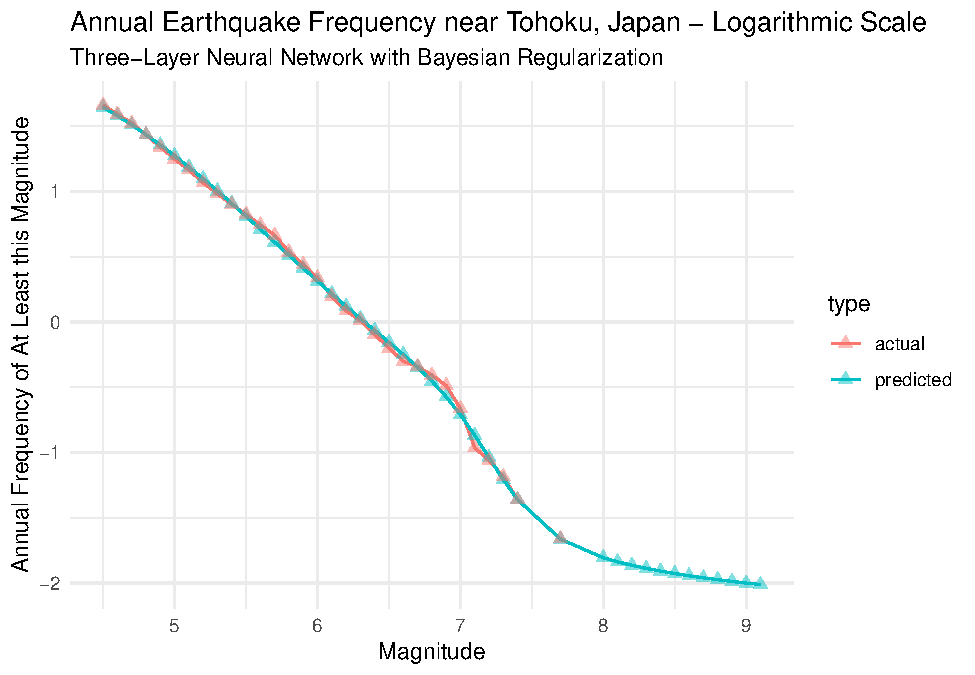
\includegraphics{earthquakes_files/figure-latex/unnamed-chunk-11-1.pdf}

\hypertarget{plot-for-brnn-returned-to-standard-scale}{%
\subsubsection{plot for brnn returned to standard
scale}\label{plot-for-brnn-returned-to-standard-scale}}

Simulating 100 networks' predictions for magnitude 9.1 with
\emph{neurons = 6}
